% #############################################################################
% This is Chapter 6
% !TEX root = ../main.tex
% #############################################################################
% Change the Name of the Chapter i the following line
\fancychapter{Integration of synthetic speech for data augmentation}
\label{chap:6}
\cleardoublepage

\section{Introduction}

% Challenge in children's speech
The continuous progress of deep learning, fueled by the abundance of extensive training datasets, has significantly improved the performances of \ac{ASR}. Nevertheless, despite these notable advancements, the recognition of children's speech poses a unique set of challenges, leading to performance disparities when compared to adult speech recognition. The inherent variability in children's speech, influenced by factors such as age, linguistic development, and articulatory differences, necessitates the acquisition of a sufficiently diverse and comprehensive dataset for the effective training of children's \ac{ASR} systems.


In an attempt to bridge this performance gap, researchers in \cite{asr-google} addressed the challenge by leveraging an in-house large dataset of children's speech, comparable in scale to an adult corpus, to train an \ac{ASR} model. The results demonstrated state-of-the-art performances, highlighting the potential of \ac{ASR} systems to effectively learn from diverse and variable children's speech data when provided with a substantial amount of training data. However, it is important to note that, in most cases, the creation of such comprehensive datasets for children's speech faces practical constraints, including ethical considerations, privacy concerns, high cost of data collection, challenges posed by children's limited attention span and inconsistent adherence to prompts during reading tasks.


In response to the challenges associated with collecting real children's speech data, an alternative strategy has emerged, involving the generation of synthetic datasets using \ac{TTS} models. \ac{TTS} offers a solution to bypass the difficulties involved in collecting and annotating real children's speech data. While some studies have explored the application of \ac{TTS} for adult \ac{ASR}, either through the direct use of synthetic speech for training or as a form of data augmentation \cite{laptev2020you, fazel21_interspeech}, synthesising children's speech introduces a unique set of challenges. The inherent substandard and imprecise pronunciation in children's speech \cite{wang2021towards} represent an obstacle, raising concerns that the direct use of synthetic data may lead to a decrease in performance \cite{wang2021towards, hu2022synt++}.

% Our Approach
In this chapter, we introduce a novel technique known as \textit{\ac{DWAT}}, to enhance children \ac{ASR} models, even in scenarios where imperfect data is employed as augmentation. Our approach involves the separate use of additional Adapter modules for synthetic data during the fine-tuning process. As demonstrated in Chapter \ref{chap:5}, the effectiveness of Adapters in bridging the gap between a source and target domain, while retaining knowledge from pre-trained models for children's speech, has been established. Therefore, we hypothesise that Adapters can be extended to mitigate the domain mismatch between real and synthetic data in the context of children's speech. To accomplish this, we propose our \ac{DWAT} approach, a two-step training procedure, drawing inspiration from the methodology introduced in \cite{fan2022draft}.


In the initial step, Adapters are exclusively trained using synthetic data, while keeping the pre-trained model frozen. This phase allows the Adapters to specialise in addressing the nuances introduced by synthetic data, including its imperfections. In the subsequent step, fine-tuning is performed, modifying both the trained Adapters and the entire model weights. During this fine-tuning process, a combination of synthetic and real data is provided to the model. Importantly, our approach introduces a crucial distinction between synthetic and real data throughout the fine-tuning process. Synthetic data passes through the Adapter layers, enabling the Adapters to handle synthetic characteristics while still contributing to the full model tuning. In contrast, real data bypasses these Adapters as it does not exhibit the imperfections inherent in synthetic data. We hypothesise that this meticulous differentiation could enable the effective use of imperfect synthetic data, ultimately leading to an enhancement in \ac{ASR} performances.


In this chapter, our objective is to address the following research questions: \textit{Is it possible to use children's synthetic speech to extend the amount of children's data? How can we control the quality and speakers’ variability?}

\section{Enhancing ASR Performance through TTS Data Augmentation}
%\ac{TTS} data augmentation
The evolution of \ac{TTS} systems, achieving human-like quality, presents a promising avenue for effective \ac{TTS}-based data augmentation in \ac{ASR}.
As exemplified in studies such as \cite{laptev2020you}, this approach entails the generation of synthetic speech from text using \ac{TTS} models and incorporating it with real speech during the training process, leading to notable performance improvements. Importantly, this data augmentation approach is not limited to well-resourced tasks and has demonstrated success even in low-resource scenarios, as illustrated in \cite{casanova2022asr}. However, despite its efficacy, \ac{TTS}-based data augmentation offers only modest improvements, primarily owing to the persistent challenge of domain mismatch between synthetic and real speech. Indeed, even with human-like qualities, some generated utterances suffer from artefacts or wrong modelisation.

To address the disparity between synthetic and real data, an approach based on shared intermediate representations has been proposed in \cite{9688218}. Instead of using Mel-scale filterbanks, this method employs discrete intermediate representations, obtained with a Vector-Quantised Wav2vec \cite{vqwav2vec}, that are shared by both the \ac{TTS} and \ac{ASR} systems. This approach has demonstrated promising results, emphasising its potential in bridging the gap between synthetic and real data in the context of \ac{ASR}. However, it is essential to note that implementing such a strategy necessitates training both the \ac{ASR} and \ac{TTS} systems from scratch. This requirement may pose challenges or may not be feasible, particularly in the context of low-resource \ac{ASR} scenarios.

% Children data selection
An alternative approach to address the domain mismatch between synthetic and real speech relies on data selection techniques, as proposed by \cite{wang2021towards}. This approach focuses on selectively choosing high-quality synthetic speech data to mitigate the challenges associated with imperfect data augmentation. The data selection process ensures that only the most reliable and accurate synthetic speech samples are incorporated during the augmentation process. One advantageous aspect of this work is that it does not necessitate more complex training for the \ac{TTS} or \ac{ASR} models. Instead, it operates as an off-the-shelf selection on top of the \ac{TTS} engine. This characteristic underscores the practicality and ease of its integration into existing \ac{TTS} systems.
In the study conducted by Wang et al. \cite{wang2021towards}, the effectiveness of using i-vector speaker-embedding cosine similarity between reference and generated utterances as a metric for data selection was demonstrated. This metric outperformed other measures, including error rate, acoustic posterior, and synthetic discriminator.

% Synth++
More recently, \cite{hu2022synt++} introduced the Synth++ framework, which employs a similar data selection approach, called rejection sampling. This rejection sampling method relies on the output of a \ac{DNN}, which is trained on a 5-dimensional features vector derived from a pre-trained \ac{ASR} model. The goal of this \ac{DNN} is to discriminate whether the data is real or synthetic. To this end, the 5-dimensional features vector for each utterance encompasses \ac{CE} loss, \ac{CTC} loss, \ac{WER}, lengths of tokens in the predicted text and the length of tokens in the target text. In addition to rejection sampling, Synth++ introduces the use of separate batch normalisation for real and synthetic data. During the training process, when synthetic data is fed into the model, it undergoes distinct normalisation layers. The incorporation of this separated normalisation has been demonstrated to significantly reduce the mismatch between real and synthetic data during training, leading to notable improvements in \ac{WER} scores.

\section{Closing the synthetic and real mismatch gap with Adapters: The Double Way Adapter Tunning approach}

\begin{figure}
    \centering
    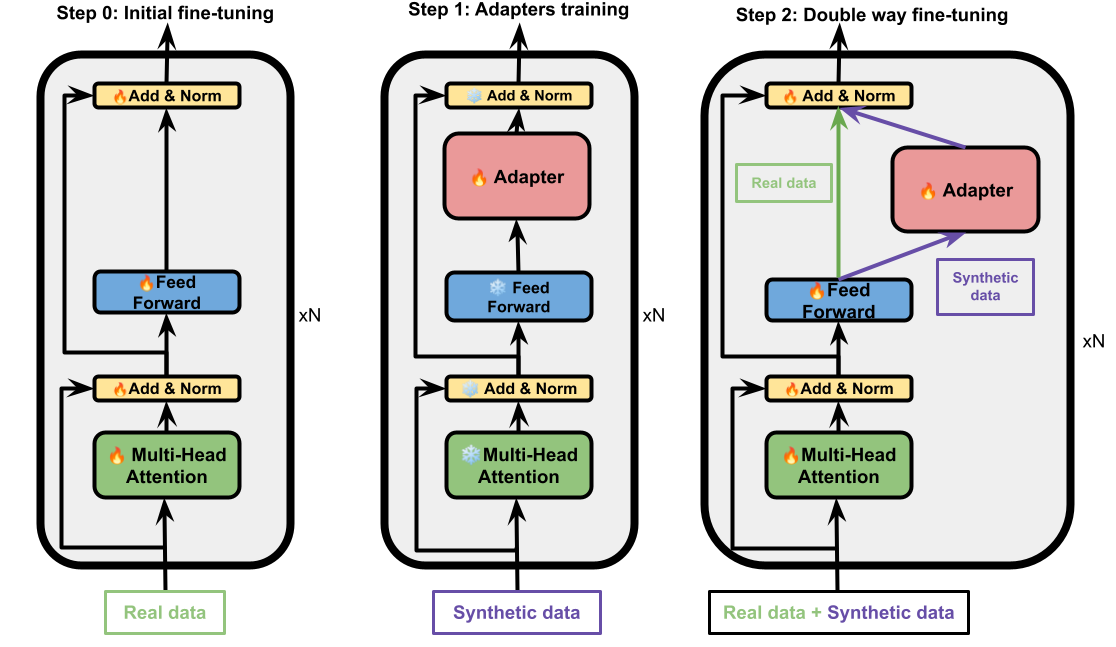
\includegraphics[width=\textwidth]{imgs/TTS_Transformer.png}
    \caption{Overview of ``Double way Adapter fine-tuning"  within the context of a Transformer model}
    \label{fig:overall_DWAT}
\end{figure}

The literature extensively documents the effectiveness of Adapters in both speech and \ac{NLP} tasks \cite{pfeiffer, philip2020monolingual, mao-etal-2022-unipelt}. Additionally, Chapter \ref{chap:5} further reinforces the positive results, demonstrating the efficacy of Adapter modules in children's \ac{ASR}. These findings highlight the role Adapters can play in addressing the mismatch between a source and target task, showcasing their ability to capture task-relevant information while preserving valuable knowledge of a frozen pre-trained model.

In alignment with these findings, \cite{fan2022draft} introduced the \ac{DRAFT} framework for children's \ac{ASR}. The authors aimed to reduce the mismatch between adult and children speech data in \ac{SSL} models. To this end, Adapters were integrated and trained within the \ac{SSL} model, followed by an additional adaptation phase where both the Adapters and the \ac{SSL} model were fine-tuned. The \ac{DRAFT} framework proved to be effective, resulting in improved performances.


Inspired by the successes of the \ac{DRAFT} framework and Synth++, our \ac{DWAT} approach integrates Adapter modules as a replacement for the separate normalisation layers in the Synth++ framework. Additionally, we incorporate the multiple-step adaptation process from the \ac{DRAFT} framework. Finally, we used filtered synthetic data, implementing a speaker-embedding cosine similarity metric to retain synthetic utterances that exhibit high-quality generation, as proposed by \cite{wang2021towards}. This combination constitutes a novel strategy to tackle the domain mismatch between real and synthetic children's speech for \ac{ASR}.

%Our primary goal is to inject external knowledge of synthetic children's speech into a pre-trained \ac{ASR} model using Adapters. This approach allows us to preserve the real children's speech knowledge acquired during pre-training while separately modelling the synthetic characteristics within the Adapter modules. Therefore, Adapters serve as a bridge, that can effectively reduce the domain mismatch between real and synthetic speech data during the training of \ac{ASR} models for children using a combination of real and synthetic data. 

%In our \ac{DWAT} framework, the objective of using Adapters is to incorporate external knowledge of synthetic children's speech into a pre-trained \ac{ASR} model. This approach enables the preservation of the real children's speech knowledge acquired during pre-training, while concurrently modeling the synthetic characteristics within the Adapter modules. Thus, Adapters act as a bridge, effectively reducing the domain mismatch between real and synthetic speech data during the training of \ac{ASR} models for children by utilizing a combination of real and synthetic data.

%Step 0
In our \ac{DWAT}  framework, as illustrated in Figure \ref{fig:overall_DWAT}, we introduce two additional steps following the standard \ac{ASR} model training with children's data (Step 0).
% Step 1
Step 1 involves the standard training of Adapter modules. While keeping the pre-trained \ac{ASR} model parameters fixed, the Adapter weights are trained on the target data, here \ac{TTS} utterances. These Adapter modules are strategically placed after the Transformer \ac{FFN} component. The goal is to learn a projection that aligns synthetic children's speech with real children's speech within each Transformer layer. This approach allows the model to retain knowledge about children's speech, while the Adapters aim to capture the inherent synthetic characteristics of the different \ac{TTS} utterances. This step is crucial, as Adapter modules require this learning process to efficiently bridge synthetic and real speech. Without this Adapter training step, the subsequent fine-tuning in Step 2 could be more challenging and less effective, as the bridge learned by Adapters has to be established concurrently with the normal fine-tuning process.

%Step2
In Step 2, we fine-tune both the Adapters trained in Step 1 and the entire pre-trained \ac{ASR} model using a mix of synthetic and real data. A pivotal aspect of our approach lies in how we handle data flow within the model. Real samples bypass the Adapter modules as they do not need further adjustments, directly passing through the original \ac{ASR} model components. In contrast, synthetic data goes through the Adapters for necessary modifications to better align with real children's speech characteristics. This differentiated treatment of data used Adapters to address the mismatch of the synthetic data, allowing the rest of the \ac{ASR} model to focus on learning normal children's characteristics. This approach has the potential to enhance the overall performance of the \ac{ASR} system.

% Inference
During the inference phase, the Adapter modules become unnecessary and are discarded since the test data only contains real samples. It is essential to note that Steps 1 and 2 can be iteratively repeated with newly generated synthetic data. However, this aspect is not investigated in this thesis and serves as a subject for future research.

% Recap
In summary, our proposed \ac{DWAT} approach uses Adapter modules to enhance the performance of a pre-trained \ac{ASR} model through the incorporation of synthetic data augmentation. This innovative methodology introduces a two-step process involving the training of Adapter and subsequent fine-tuning of the \ac{ASR} model with a mix of synthetic and real data using Adapters to bridge the domain gap between real and synthetic children's speech.


\section{Overview of the automatic speech recognition and text-to-speech systems}
\label{section:SOA}
\subsection{Transformer architecture for ASR}

For this experiment, we used a pre-trained Transformer model\footnote{https://huggingface.co/speechbrain/asr-transformer-transformerlm-librispeech/tree/916c9ff} based on the SpeechBrain toolkit \cite{speechbrain} as the \ac{ASR} component. The choice of the Transformer architecture was motivated by the positive results obtained for children's \ac{ASR} in previous chapters. We will not delve into the details of the Transformer architecture here, as a comprehensive explanation was provided in Section \ref{sec:trans_archi}. For this experiment, the model was trained on the LibriSpeech dataset \cite{librispeech}, comprising 12 Encoder Transformer layers and 6 Decoder Transformer layers, each with a dimension of 512. For training, we employed a combination of \ac{Seq2Seq} and \ac{CTC} loss functions, with respective weights of 0.7 and 0.3. Additionally, we integrated a Transformer language model trained on a 10 million-word corpus of transcriptions from the LibriSpeech dataset.
It is essential to note that this particular instantiation of the Transformer model is different from the one employed in the previous chapters of our study. 

%In our experiments, we employed the SpeechBrain toolkit \cite{speechbrain} for the \ac{ASR} component of our system, using a pre-trained Transformer model\footnote{https://huggingface.co/speechbrain/asr-transformer-transformerlm-librispeech}. This model has trained on the LibriSpeech dataset \cite{librispeech} and comprises 12 Encoder layers and 6 Decoder layers, each with a dimension of 512. It is noteworthy, that is Transformer model is different from the one used in previous Chapters. A mix of \ac{Seq2Seq} and \ac{CTC} loss were used with respective weights of 0.7 and 0.3. Additionally, we integrated a Transformer language model trained on a 10 million-word transcription of Librispeech.

\subsection{Multi-speaker text-to-speech: YourTTS}

\begin{figure}
    \begin{center}
        \includegraphics[scale=0.4]{imgs/YourTTS.png}
        \caption{Architecture of the YourTTS model\protect\footnotemark}
        \label{fig:YourTTS}
    \end{center}
\end{figure}

In this work for the \ac{TTS} component, we used the pre-trained YourTTS model\footnote{https://coqui.ai/blog/tts/yourtts-zero-shot-text-synthesis-low-resource-languages} proposed by \cite{casanova2022yourtts} based on the  Coqui toolkit. YourTTS is a zero-shot multi-speaker and multilingual \ac{TTS} system that is built upon the \ac{VITS} model. It incorporates several novel modifications to enable zero-shot multi-speaker and multilingual synthesis. An overview of the YourTTS architecture is presented in Figure \ref{fig:YourTTS}.
% General description of YourTTS
YourTTS features a 10-layer Transformer-based text Encoder with 196 hidden channels. This Encoder, adaptable for multilingual use, employs a 4-dimensional language embedding concatenated with the embedding of each input character. However, for the purpose of our experiment, we exclusively use the English language. The Decoder comprises four affine coupling layers \cite{45819}, each incorporating four WaveNet blocks \cite{45774} to ensure high-quality speech generation. The model also uses the HifiGAN vocoder \cite{kong2020hifi}. Notably, YourTTS adopts an end-to-end approach, connecting the vocoder to the \ac{TTS} model through a \ac{VAE} \cite{VAE}.
\footnotetext{Figure taken from https://coqui.ai/blog/tts/yourtts-zero-shot-text-synthesis-low-resource-languages} % Just a trick to put it to the correct location


To enhance its capabilities as a multi-speaker and zero-shot \ac{TTS} system, YourTTS integrates a speaker Encoder, specifically the \ac{H/ASP} speaker Encoder \cite{heo2020clova}, generating 512-dimensional speaker embeddings for each utterances. This speaker Encoder model is compromising a \ac{CNN} layers, followed by four Resnet layers \cite{targ2016resnet}, an attentive statistic pooling and an output linear layer. These embeddings serve as reference speakers for the \ac{TTS} model, enabling zero-shot multi-speaker capabilities. To this end, the authors conditioned all affine coupling layers of the flow-based Decoder, the posterior Encoder, and the vocoder on external speaker embeddings. Additionally, a \ac{SCL} is added to the final loss to further enhance the multi-speaker ability of the model. The \ac{SCL} is formally expressed as follows:

\begin{equation}
    L_{SCL} = \frac{-\alpha}{n} \cdot \sum_{i}^{n} cos\_sim(\phi(g_i), \phi(h_i))
\end{equation}

where let $\phi(\cdot)$ be the function outputting the speaker embeddings, $cos\_sim$ is the cosine similarity function, $\alpha$ is a positive real number controlling the influence of the \ac{SCL} in the final loss, $n$ is the batch size and $g$ and $h$ represent, respectively, the ground truth and the generated speaker audio.

The YourTTS model was trained using three languages: English with VCTK \cite{veaux2016superseded}, Brazilian Portuguese with TTS-Portuguese Corpus \cite{casanova2022tts}, and French with the French set of the M-AILABS dataset \cite{mailabs}. This training corpus totalled 229 hours of speech data and involved 115 speakers. For a more in-depth understanding of the YourTTS architecture and training process, detailed information can be found in the original paper \cite{casanova2022yourtts}.


\section{Experimental setup}
\label{section:methods}

%\subsection{Real speech corpus}
%\begin{table}[h!]
%\caption{My Science Tutor Children Speech Corpus statistics}

%\begin{center}
%\begin{tabular}{r|c|c|c}
%\hline
% & Training & Validation     & Test   \\ \hline
%\# of utterances & 60897   & 10044    & 4079  \\ 
%\# of speakers & 566   & 79    & 91  \\ 
%\# of hours & 113   & 18    & 13  \\ \hline
%\end{tabular}
%\label{tab:statistics}
%\end{center}
%\end{table}
This experiment uses the My Science Tutor (MyST) Children Speech Corpus, as the "Real" children'speech set. We used the Myst dataset here as it was employed in prior experiments conducted on this dataset within the context of this thesis, as detailed in Table \ref{tab:statistics_myst}. For a more comprehensive understanding of the MyST corpora, additional details are provided in Section \ref{section:children_corpora}.


\subsection{Synthetic data}
% Finetune YourTTS with MyST train set
To address the potential performance gap caused by the YourTTS model being trained solely on adult data and never exposed to children's data, we initiated the process by fine-tuning the YourTTS model using the MyST training set. In this study, two \ac{TTS} systems were developed, each with distinct parameter settings, to examine their respective performances and output quality under varying conditions. The two \ac{TTS} systems, namely TTS$_1$ and TTS$_2$, were developed with distinct parameter settings. The first model, TTS$_1$, underwent fine-tuning for 250 epochs, without incorporating the speaker Encoder \ac{SCL} loss. In contrast, the second system, TTS$_2$, was fine-tuned for 50 epochs, incorporating the speaker Encoder \ac{SCL} loss. This incorporation should improve the alignment between the generated speech and the reference speaker embedding provided to the model. These variations in training strategies enable a thorough examination of the model's performance and output quality under varying conditions,

% Use randomly selected speaker utterances from the training set, d-vector -> TTS
The first \ac{TTS} model, TTS$_1$, was used to generate 300 hours of synthetic data referred to as \textit{Synth$_1$}. The second \ac{TTS} model, TTS$_2$, was employed to generate a larger volume of synthetic data, up to 1,000 hours, denoted as \textit{Large Synth$_2 $}. To compare the performance of TTS$_1$ and TTS$_2$, a subset of 300 hours was extracted from the \textit{Large Synth$_2$} dataset, called \textit{Synth$_2$}. The full 1,000-hour set was exclusively used to evaluate the impact of different amounts of synthetic data on the performances of our \ac{DWAT} approach.

The speech synthesis process using the YourTTS model requires a text transcription and a speaker-embedding vector to generate a synthetic utterance. Therefore, to generate an utterance in both \textit{Synth$_1$} and \textit{Large Synth$_2$}, we randomly selected two utterances from the Myst training set, one designated for extracting the speaker embedding and the other exclusively used for its text transcription. The Myst training set comprises 60,897 utterances, therefore resulting in a vast pool of potential combinations, totaling 3,708,444,609 unique combinations. This extensive range of possibilities was strategically harnessed to introduce a deliberate mismatch between the selected speaker embeddings and their associated transcriptions. This intentionally large range of possibilities served as a mechanism to infuse novel variability into the synthetic data, thereby introducing characteristics not present in the original real corpus.

The decision to use MyST transcriptions for generating synthetic data was driven by the aim to expose the \ac{TTS} model to the unique transcription style present in the MyST dataset. This style encompasses elements such as ``UM" hesitations. By adopting this strategy, we intended to enhance the model's ability to learn and reproduce the specific transcription characteristics of the MyST data.

To ensure the quality of the synthetic utterances in \textit{Synth$_1$} and \textit{Large Synth$_2$}, we extended the approach proposed by \cite{wang2021towards}, which involves using cosine similarity between the speaker embeddings of the reference and synthetic utterances as a data selection criterion. Instead of using i-vector speaker embeddings, we opted for an x-vector approach and employed a different speaker embedding extractor than the one used by the YourTTS model (to prevent conflicts with the \ac{SCL} loss). Specifically, we used a pre-trained ECAPA-TDNN \cite{desplanques20_interspeech} based x-vector extractor trained on VoxCeleb\footnote{https://huggingface.co/speechbrain/spkrec-ecapa-voxceleb}. To this end, during the generation process, we applied a cosine similarity threshold of 0.75 to discard all poorly generated synthetic utterances. While exploring data selection mechanisms, we considered the rejection sampling method suggested by Synth++ \cite{hu2022synt++} but found it unsatisfactory, ultimately opting for speaker-embedding similarity. To comprehensively evaluate the impact of this data selection, we also created \textit{Unfiltered Synth$_1$} and \textit{Unfiltered Synth$_2$}, two 300-hour corpora of synthetic data generated without using speaker embedding data selection, created with TTS$_1$ and TTS$_2$, respectively.

\subsection{Experiments}
The evaluation of our \ac{DWAT} approach involved a comprehensive series of experiments, systematically comparing its performance with existing methods. The initial phase focused on the development of baseline models, by fine-tuning a pre-trained adult model to children's speech. This fine-tuning used exclusively the \textit{Real} data for 20 and 25 epochs, corresponding to step 0 in Figure \ref{fig:overall_DWAT}.

Subsequent assessments involved the exploration of \ac{TTS} data augmentation by combining \textit{Synth$_1$} and \textit{Synth$_2$} data with the \textit{Real} data. To evaluate the impact of data filtering, we assess the results of filtered \ac{TTS} data augmented with their unfiltered counterparts, denoted as \textit{Unfiltered Synth$_1$} and \textit{Unfiltered Synth$_2$}. Additionally, we analyse the performance of models trained solely on the filtered synthetic data, aiming to discern the presence of a mismatch between the \textit{Real} and synthetic domains. In addition, we conducted an evaluation of a two-step adaptation process. Initially, the model is fine-tuning with synthetic data only, followed by a subsequent fine-tuning phase exclusively with the \textit{Real} data. All models involved in these data augmentation experiments underwent training for 20 epochs.

Moreover, our exploration delved into the incorporation of double-way normalisation, where distinct normalisation layers within the Transformer architecture were applied to synthetic data during the fine-tuning process. This concept was inspired by the methodology introduced in Synth++ \cite{hu2022synt++}. In one scenario, fine-tuning was conducted directly from the adult model for 20 epochs, incorporating both filtered synthetic and \textit{Real} data. This specific configuration is denoted as \textit{Norm double-way from adult}. To facilitate a comprehensive comparison with our \ac{DWAT} approach, we introduced an alternative scenario where the double-way normalisation model was trained for 5 epochs, using the baseline model as a starting point for the fine-tuning. This particular configuration is referenced as \textit{Norm double-way from children}.

Finally, we implemented our \textit{\ac{DWAT}} approach, training the models for 5 epochs with the baseline model as initialisation. In section, \ref{section:exp_DWAT}, we will delve into the exploration of various hyper-parameter configuration's influence on the \ac{DWAT} framework.

\section{Results and discussion}
\label{section:exp_DWAT}

\subsection{Comparison with existing approaches}

\begin{table}[t]
\centering
\begin{tabular}{ccc}
\hline
 Method & TTS$_1$ & TTS$_2$  \\ \hline
\multicolumn{1}{l}{\textit{Real (20 epochs)}} & \multicolumn{2}{c}{12.99\%}\\ 
\multicolumn{1}{l}{\textit{Real (25 epochs)}} & \multicolumn{2}{c}{13.15\%}\\ \hline
\multicolumn{1}{l}{\textit{Real} + Unfiltered \textit{Synth}}  &   13.41\%  & 13.24\% \\ 
\multicolumn{1}{l}{\textit{Real} + \textit{Synth} \cite{wang2021towards}} & 13.09\% & 12.98\% \\
\multicolumn{1}{l}{\textit{Synth} alone}    & 40.58\%  & 40.21\%  \\
\multicolumn{1}{l}{Two step adaptation}    & 13.49\%  & 13.46\%  \\
\hline
\multicolumn{1}{l}{Norm double-way (from adult)} & 12.89\% & 13.04\% \\ 
\multicolumn{1}{l}{Norm double-way (from children)} & 13.56\% & 13.87\% \\ \hline
\multicolumn{1}{l}{DWAT (Ours)} &\textbf{ 12.42\%} & \textbf{12.31\%} \\ \hline
\end{tabular}

\caption{Results of the different use of synthetic data augmentation approaches in WER. Collomn TTS$_1$ and TTS$_2$ correspond to the respective model used to generate the synthetic data.}
\label{tab:res_DWAT}
\end{table}

% Baseline
Table \ref{tab:res_DWAT} presents the results of the various approaches. The baseline models, achieved by fine-tuning an adult model on children's speech using \textit{Real} data, yielded a \ac{WER} score of 12.99\%. However, extending the training to 25 epochs led to overfitting, resulting in a subsequent reduction in performance with a \ac{WER} of 13.15\%.


Moving to the impact of synthetic data augmentation, incorporating filtered synthetic data (\textit{Real +  Synth}) as opposed to the unfiltered counterpart (\textit{Real + Unfiltered Synth}), revealed a notable 2\% relative \ac{WER} improvement when using the filtered versions. However, relying solely on filtered \ac{TTS} speech (\textit{Synth} alone) without any \textit{Real} data resulted in a was found to be ineffective with around 40\% \ac{WER} on the \textit{Real} test set for both TTS$_1$ and TTS$_2$. This discrepancy underscores the considerable domain mismatch between real and synthetic data, emphasising the imperative need for further approaches to mitigate this gap in the context of synthetic data augmentation.

Furthermore, we explored the two-step adaptation process, wherein the adult model was initially fine-tuned using only filtered \textit{Synth} data, followed by subsequent fine-tuning with only \textit{Real} speech. However, the results indicated a slight decrease in performance in both cases compared to the baseline model, with \ac{WER} scores of 13.49\% and 13.46\%, for respectively TTS$_1$ and TTS$_2$. This decline could be attributed to the potential gap between the characteristics of \ac{TTS} data, which may be more pronounced than the gap between adult and children data.


% Double-norm 
During our experiments, the use of double batch normalisation proved to be ineffective in enhancing the performance of the baseline model. On the contrary, it resulted in a 5\% relative decrease in \ac{WER}  when evaluated with the baseline model as initialisation (from children). It is worth noting that, when training from the adult model, the results remained consistent with those of the baseline models, showcasing no observed improvement. These outcomes underscore the limitations of double batch normalisation in addressing the domain mismatch between real and synthetic speech data within a Transformer model. This emphasises the significance of exploring alternative strategies to effectively bridge this gap.


% Adapter Double-way
Our proposed \ac{DWAT} approach, using the baseline model as the initial step (step 0), emerged as the most effective among all the methods examined. It demonstrated a notable 4\% and 5\% relative improvement in \ac{WER} over the baseline when evaluated on \textit{Synth$_1$} and \textit{Synth$_2$} respectively. Additionally, we observed that our approach, while training 5 additional epochs, did not lead to overfitting, especially compared to longer training on the \textit{Real} set (\textit{Real 25 epoch}), showcasing its potential in mitigating the challenges posed by domain mismatch in the context of synthetic data augmentation for children \ac{ASR}.


\subsection{Influence of synthetic number of hours}
\begin{table}[t]
\centering
\begin{tabular}{cc}
\hline
 Amount of TTS data & WER $\downarrow$   \\ \hline
\multicolumn{1}{c}{0h} & 12.99\% \\ \hline
\multicolumn{1}{c}{10h}  &   12.73\%   \\ 
\multicolumn{1}{c}{50h}    & 12.54\%   \\ 
\multicolumn{1}{c}{100h} & 12.49\%  \\ 
\multicolumn{1}{c}{300h} & \textbf{12.31\%}  \\ 
\multicolumn{1}{c}{600h} & 12.57\%  \\ 
\multicolumn{1}{c}{1000h} & 13.14\%  \\ \hline

\end{tabular}

\caption{Results of the different number of hours influence in our DWAT approach with \textit{Large Synth$_2$} data}
\label{tab:hours}
\end{table}

%Time experiments
Given the potential of our approach to generating a theoretically ``infinite" amount of \ac{TTS} data, we aimed to evaluate the impact of varying synthetic data quantities on the efficacy of the \ac{DWAT} approach. To this end, we assess the influence of different quantities of synthetic data taken from \textit{Large Synth$_2$}, as detailed in Table \ref{tab:hours}.
The findings from our investigation reveal that utilising a small quantity of synthesised speech, ranging from 10 to 50 hours, results in limited improvements in \ac{ASR} performance. Conversely, an excessive volume of \ac{TTS} data, spanning from 600 to 1,000 hours, has the potential to introduce undesirable noise into the system. Notably, only the configuration with 1,000 hours failed to improve the baseline score of 12.99\%. Consequently, achieving an optimal equilibrium becomes crucial. In our experiment, we found that this equilibrium of synthetic speech fell within the same range as the number of hours available for real speech, around 100 to 300 hours. This balance aims to enhance the robustness of \ac{ASR} performance with new variabilities while concurrently preventing the introduction of excessive noise, thereby maximising the effectiveness of the \ac{DWAT} approach.

\subsection{Impact of DWAT different hyperparameter configurations}
\label{sec:hyperparameter}
\begin{table}[t]
\centering
\begin{tabular}{cccc}
\hline
 Location &  Bottleneck size &  5 epochs &  20 epochs     \\ \hline
\multicolumn{1}{c}{Encoder} & 64 & 12.58\% & 12.24\% \\ 
\multicolumn{1}{c}{Encoder} & 128 &  12.31\% & 12.45\%  \\ 
\multicolumn{1}{c}{Encoder} & 256  & \textbf{12.25\%} & 12.32\%  \\ 
\multicolumn{1}{c}{Encoder} & 1024 & 12.42\% & \textbf{12.22\%} \\ 
\multicolumn{1}{c}{Encoder} & 2048 & 12.57\% & 12.47\% \\ \hline
\multicolumn{1}{c}{Encoder-Decoder} & 128 & 12.45\% & 12.48\% \\ \hline
\multicolumn{1}{c}{Skip step 0} & 256 & 12.30\% & - \\ 
\multicolumn{1}{c}{Skip step 0 and 1} & 256 & 13.28\% & - \\ \hline

\end{tabular}

\caption{Results of the different configurations of Adapter double-way approach on 300h of \textit{Synth$_2$}}
\label{tab:config_hparams}
\end{table}
To further evaluate the robustness of our approach, we conducted experiments with various hyperparameter configurations of \ac{DWAT}. This extensive analysis involved exploring different Adapters's bottleneck sizes, ranging from 64 to 2048, varying the number of final fine-tuning training epochs (5 and 20), investigating the integration of Adapters in the Decoder of the transformer model, and performing an ablation study by skipping step 0 and both steps 0 and 1 in the \ac{DWAT} process.

% Best config
The results of the different configurations are summarised in Table \ref{tab:config_hparams}. These results provide insights into the optimal configuration, revealing that the most effective setup consists of  Adapters with a hidden dimension size of 1024, placed in the Encoder only, coupled with 20 training epochs for the final fine-tuning. This configuration resulted in a remarkable 6\% relative \ac{WER} reduction compared to the baseline. Notably, all configurations demonstrated superior performance to the baseline, underscoring the overall effectiveness of our \ac{DWAT} approach.

% Other results
Furthermore, our results indicate that extending the training period in was particularly advantageous for larger Adapter bottleneck sizes, demonstrating no signs of overfitting. Moreover, the integration of Adapters into the Decoder did not lead to a significant improvement in results. This outcome can be attributed to the higher acoustic variability typically captured in the Encoder, coupled with the fact that the same transcriptions from the Myst dataset were used for synthetic speech utterances, thereby diminishing the potential for further improvement in the Decoder. Lastly, skipping step 0 (initial children pre-training) did not result in a significant degradation in performance. However, when both step 0 and step 1 (initial pre-training and Adapter pre-training) were skipped, performance degradation occurred, underscoring the critical role of the Adapter pre-training phase (step 1) in achieving good performances.

\subsection{Extension DWAT to the Conformer architecture}
\begin{figure}
    \centering
    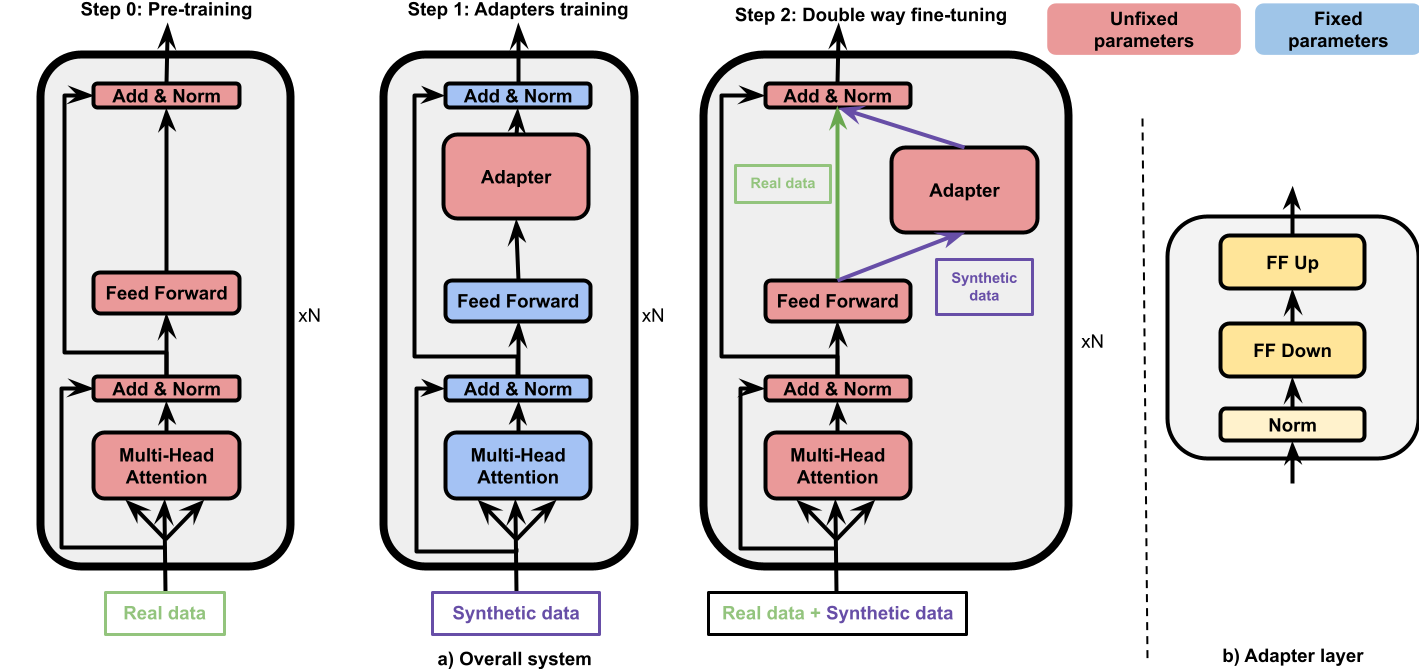
\includegraphics[width=\textwidth]{imgs/Overall_system.png}
    \caption{Overview of ``Double way Adapter fine-tuning"  within the context of a Conformer architecture}
    \label{fig:TTS_conformer}
\end{figure}

Building upon the positive outcomes observed in previous chapters, where the Conformer architecture showcased superior performance compared to the regular Transformer in children's \ac{ASR}, and considering the efficacy of Adapters in the Conformer architecture, we decided to assess the performance of our \ac{DWAT} within the Conformer architecture. Additionally, since Synth++ \cite{hu2022synt++} was initially designed for the Conformer architecture, we opted to evaluate the Synth++ double-normalisation layers compared to our \ac{DWAT} in this setting. 

Due to the demonstrated effectiveness of the \ac{TPA} configuration for the Conformer model, we chose to implement our \ac{DWAT} framework within the Conformer architecture using two Adapters per layer, specifically, one for each \ac{FFN} module—in parallel. The integration of our \ac{DWAT} framework within the Conformer using \ac{TPA} is illustrated in Figure \ref{fig:TTS_conformer}.

In this experiment, we employed the same pre-trained adult Conformer model as employed in the preceding chapters. This model consists of 12 layers of Conformer in the Encoder, followed by 6 Transformer layers in the Decoder, all with a hidden dimension of 512. The same language model was used and aligns with the experiments conducted in the Transformer model detailed in the preceding sections. In light of the insights derived from the exploration of hyperparameters in Section \ref{sec:hyperparameter}, we chose Adapters with a hidden dimension size of 512, solely in the Encoder and using the \ac{TPA} configuration. Regarding training, both Step 0 and Step 1 were trained for 30 epochs, while Step 2 was only 10 epochs.

\begin{table}[h]
    \centering
    \begin{tabular}{lr}
        \toprule
        Method & WER Score $\downarrow$ \\
        \midrule
        Adult Frozen model & 21.75\% \\
        \textit{Real} only & 12.28\% \\ \hline
        \textit{Unfiltered Synth$_2$} & 37.85\% \\
        \textit{Unfiltered Synth$_2$} + \textit{Real} & 12.30\% \\ 
        \textit{Synth$_2$} alone & 31.72\% \\
        \textit{Synth$_2$}+ \textit{Real} & 12.02\% \\ 
        Two-step adaptation & 12.51\% \\ \hline
        Synth++ (Norm double way) & 11.80\% \\
        DWAT & \textbf{11.64\%} \\
        \bottomrule
    \end{tabular}
    \caption{Scores for the different methods of synthetic data augmentation within the Conformer architecture}
    \label{tab:DWAT_conformer}
\end{table}

The results obtained from the extension of \ac{DWAT} to the Conformer architecture are presented in Table \ref{tab:DWAT_conformer}. The frozen adult model achieved a \ac{WER} score of 21.75\%. When considering only real data (\textit{Real} only), the \ac{WER} score improved significantly to 12.28\%. Which is already outperforming the best results of the Transformer.

When using unfiltered synthetic data alone (\textit{Unfiltered Synth$_2$}) method, it resulted in a higher \ac{WER} score of 37.85\%, showcasing, once again, the mismatch between synthetic and real data. However, when combined with real data (\textit{Unfiltered Synth$_2$} + \textit{Real}), the results are closer to the real baseline with a \ac{WER} score of 12.30\%. Similarly, using the filtered \textit{Synth$_2$} alone resulted in a \ac{WER} score of 31.72\%, but when combined with real data (\textit{Synth$_2$} + \textit{Real}), the \ac{WER} score decreased significantly to 12.02\%. This differs from the results observed in the Transformer architecture, as in the Conformer scenario, data filtering has been able to improve the \ac{WER} score compared to the baseline.
Additionally, similarly to the Transformer, the two-step adaptation method yielded a \ac{WER} score of 12.51\%, falling behind the baseline score. 

Further insights into the performance of the more sophisticated methods are provided in the context of the Conformer architecture. Specifically, the Synth++ method, which incorporates separated batch normalisation within each Convolution module for \ac{TTS} data, achieved a \ac{WER} score of 11.80\%. This contrasts with the results observed in the Transformer experiment, highlighting the efficiency of this approach specifically within Conformer models. On the other hand, the \ac{DWAT} method consistently outperformed all other methods, showcasing a remarkable \ac{WER} score of 11.64\%. These findings emphasise the effectiveness of both the Synth++ and \ac{DWAT} methods in enhancing the Conformer architecture's performance on the given task.

However, it is important to highlight that while both Synth++ and \ac{DWAT} demonstrate efficacy within the Conformer setup, the \ac{DWAT} approach consistently outperforms other methods in both Transformer and Conformer configurations. This consistent superiority underscores the relevance and robustness of the \ac{DWAT} approach in improving the overall performance of the children \ac{ASR} models across different architectures.

In summary, the experimental results demonstrate the effectiveness of leveraging synthetic data, real data, and advanced adaptation methods within the Conformer architecture. The \ac{DWAT} method, in particular, stands out as the most successful approach in minimising the \ac{WER}.


\section{Summary and discussion}
\label{section:conclusions_TTS}

In this chapter, we aimed to answer to the following research questions: \textit{Is it possible to use children's synthetic speech to extend the amount of children's data? How can we control the quality and speakers’ variability?}

% Summary 
We provide positive responses to both research questions through the introduction of our novel methodology: the Double Way Adapter Transfer procedure, which combines Adapters and synthetic data augmentation for children's speech recognition. Our two-phase training strategy consists of the initial training of Adapter modules using synthetic data, followed by the fine-tuning of Adapters and the entire model weights. Importantly, during this fine-tuning process, real data bypasses the Adapter modules. This distinctive dual-pathway approach resulted in notable improvement over baseline and previous techniques across various configurations. Importantly, our approach demonstrated robustness across different \ac{ASR} architectures, \ac{TTS} model fine-tuning parameters, Adapter sizes, number of epochs, and varying amounts of synthetic data. Furthermore, our study showcases the controllability of \ac{TTS} output quality without necessitating direct modifications of the \ac{TTS} model. This filtering process, performed before applying the \ac{DWAT}, is achieved through the use of pre-trained x-vectors speaker embeddings and cosine similarity metrics between reference and generated utterances. This approach, improved from previous work where only i-vectors were used\cite{wang2021towards}, allows the use of synthetic data which align more closely with desired characteristics of real children's speech, contributing to a more controlled augmentation process.

% Discussion
The promising performances observed with the \ac{DWAT} pave the way for future research avenues. One potential avenue involves adopting an iterative methodology, dynamically incorporating newly generated \ac{TTS} data while adjusting the proportion of real data and repeating the operation as needed. This iterative fine-tuning approach could potentially provide further insights into the interaction between synthetic and real data, offering opportunities to refine and optimise the training process for improved children's \ac{ASR} models.
Another avenue of exploration could be to extend the \ac{DWAT} framework to domains beyond the synthetic and real speech data. Investigating the adaptability and effectiveness of \ac{DWAT} in diverse domains, such as adult and children's speech domains could be an interesting first step towards this direction.
Furthermore, considering the rapid evolution of the \ac{PETL} approaches, the exploration of new modules as replacements for Adapters represents a new research direction. An initial step in this direction will be explored in the upcoming chapter, where we conduct a thorough evaluation of different \ac{PETL} alternatives. The goal is to identify novel strategies for enhancing children's \ac{ASR} systems.